% ================================================================
% Results Chapter
% Presents the experimental findings for both environments across
% the three agent conditions. Content is objective and descriptive;
% deeper interpretation is deferred to Chapter 5 (Discussion).
% ================================================================

\chapter{Results}
\label{ch:results}

This chapter presents the experimental results. We evaluate three configurations across two Gymnasium environments, with each repeated using five random seeds. The configurations under comparison are:

\begin{itemize}
    \item \textbf{Condition~A (Model-Free Actor-Critic)}: a baseline actor-critic agent training on real environment interactions.
    \item \textbf{Condition~B (Imagination AC, standard MSE)}: an imagination-augmented actor-critic using standard MSE losses.
    \item \textbf{Condition~C (Imagination AC, Symlog MSE)}: an imagination-augmented actor-critic using symlog-transformed losses for the critic and reward prediction.
\end{itemize}

\noindent We present learning curves, critic loss stability, and world model prediction accuracy for each environment. Shaded regions in learning-curve plots denote the standard deviation across the five seeds.


% ================================================================
\section{CartPole-v1 Results}
\label{sec:cartpole-results}
% ================================================================

CartPole-v1 is a simple balancing task with a constant $+1$ reward per time
step and a maximum episode length of 500. All agents were trained for
100\,000 environment steps.

% ---------------------------------------------------------------
\subsection{Learning Curves}
\label{subsec:cartpole-learning}
% ---------------------------------------------------------------

Figure~\ref{fig:cartpole-learning} shows the mean episodic return over
training for each condition. The Model-Free baseline (Condition~A) rises
steadily and plateaus at approximately 350 return. Condition~B
(Imagination, standard MSE) displays higher sample efficiency in the early
phase of training, reaching a mean return of roughly 400 by 60\,000 steps,
but subsequently plateaus and does not improve further. Condition~C
(Imagination, Symlog MSE) starts comparatively slower than Condition~B but
continues to improve beyond the 60\,000-step mark and ultimately achieves
the highest final return of approximately 430.

\begin{figure}[H]
    \centering
    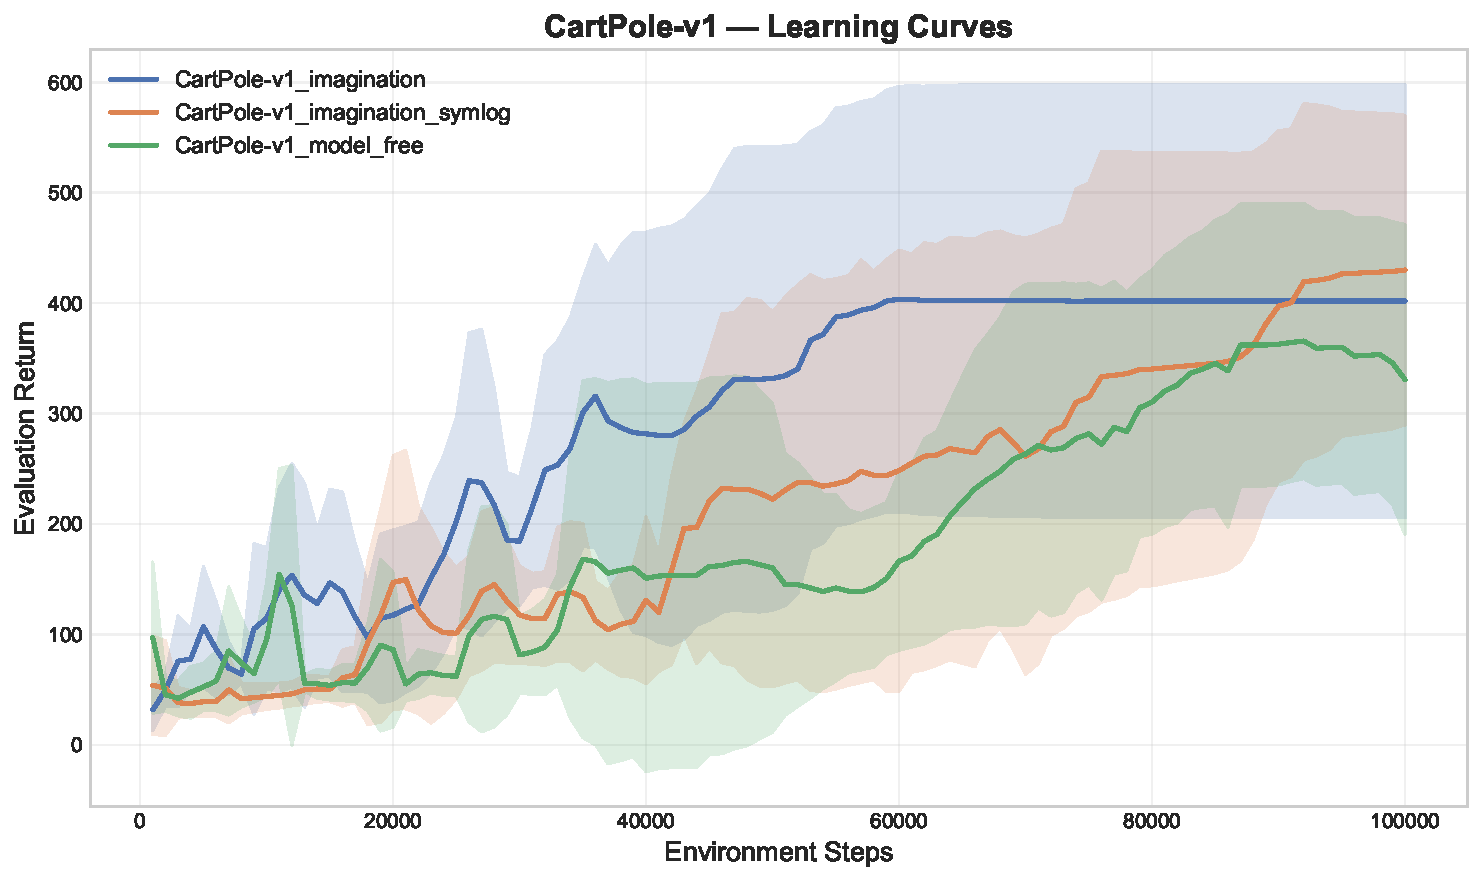
\includegraphics[width=0.85\textwidth]{figures/CartPole-v1_learning_curves.pdf}
    \caption{CartPole-v1 learning curves: mean episodic return ($\pm 1$
             standard deviation) over 100\,000 environment steps for each
             agent condition.}
    \label{fig:cartpole-learning}
\end{figure}

% ---------------------------------------------------------------
\subsection{Critic Loss Stability}
\label{subsec:cartpole-critic}
% ---------------------------------------------------------------

Figure~\ref{fig:cartpole-loss} compares the critic loss trajectories of the
two imagination-augmented conditions. Condition~B (standard MSE) exhibits a
pronounced loss explosion towards the end of training, with the critic loss
escalating to approximately $5 \times 10^{11}$. In contrast, Condition~C
(Symlog MSE) maintains a near-zero critic loss throughout the entire
training run, with no observable instability.

\begin{figure}[H]
    \centering
    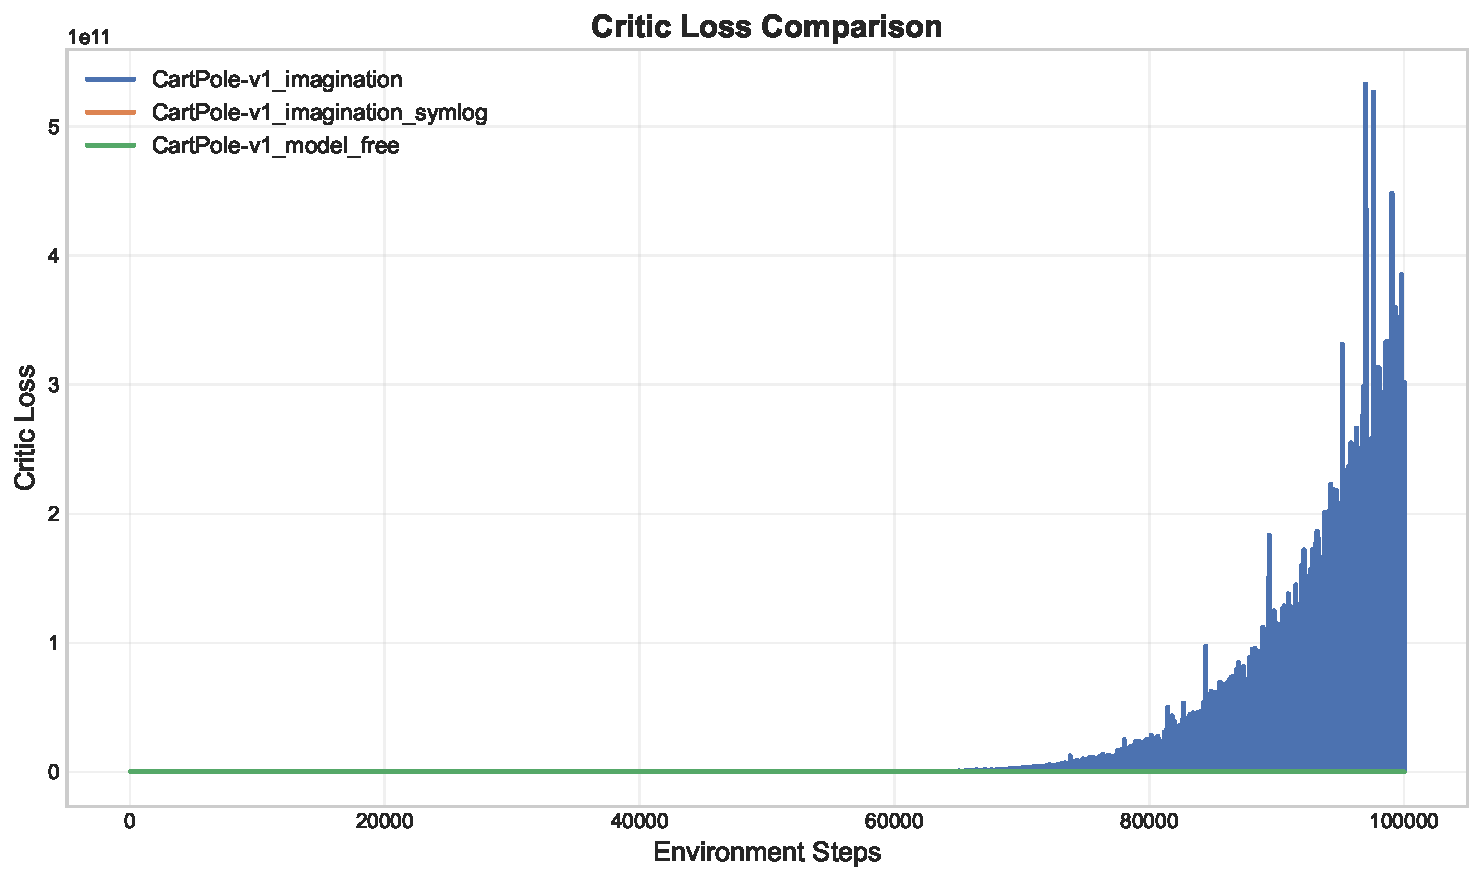
\includegraphics[width=0.85\textwidth]{figures/CartPole-v1_loss_comparison.pdf}
    \caption{CartPole-v1 critic loss comparison between the two
             imagination-augmented conditions over 100\,000 environment
             steps. Note the divergent $y$-axis scale caused by the loss
             explosion in Condition~B.}
    \label{fig:cartpole-loss}
\end{figure}

% ---------------------------------------------------------------
\subsection{World Model Accuracy}
\label{subsec:cartpole-wm}
% ---------------------------------------------------------------

Figure~\ref{fig:cartpole-wm} displays the world model prediction errors for
both dynamics (next-state prediction) and reward prediction. Both
imagination-augmented conditions learn the CartPole dynamics rapidly, with
dynamics prediction error falling to near zero early in training. Reward
prediction error is similarly negligible for both conditions, which is
expected given that CartPole-v1 issues a constant $+1$ reward at every
non-terminal step.

\begin{figure}[H]
    \centering
    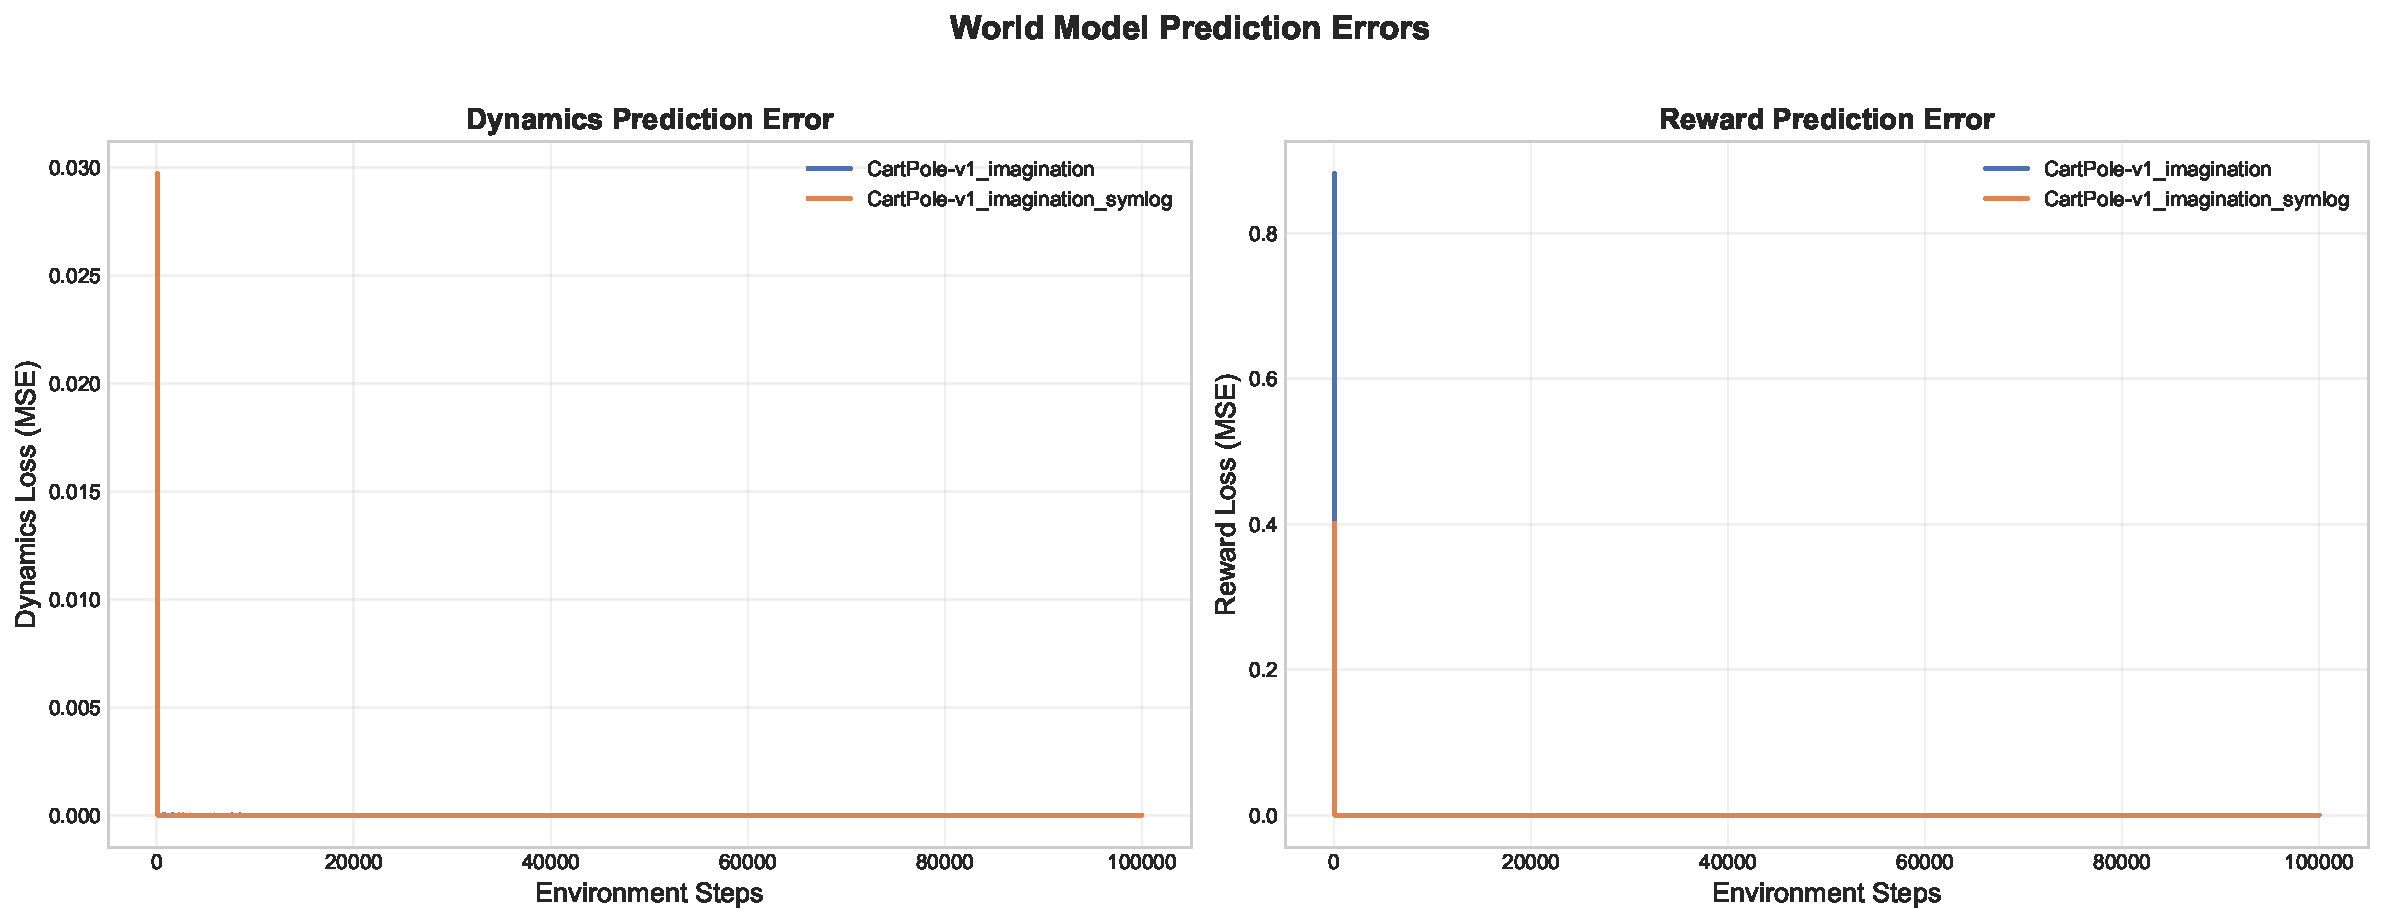
\includegraphics[width=0.85\textwidth]{figures/CartPole-v1_world_model_error.pdf}
    \caption{CartPole-v1 world model prediction error: dynamics MSE and
             reward MSE for Conditions~B and~C over 100\,000 environment
             steps.}
    \label{fig:cartpole-wm}
\end{figure}


% ================================================================
\section{LunarLander-v3 Results}
\label{sec:lunar-results}
% ================================================================

LunarLander-v3 is a continuous-control landing task with a shaped reward
signal that spans a wide numerical range (from large negative penalties for
crashing to positive bonuses for a controlled touchdown). All agents were
trained for 300\,000 environment steps.

% ---------------------------------------------------------------
\subsection{Learning Curves}
\label{subsec:lunar-learning}
% ---------------------------------------------------------------

Figure~\ref{fig:lunar-learning} shows the mean episodic return for each
condition. The Model-Free baseline (Condition~A) converges to a stable mean
return of approximately $-140$. Condition~C (Imagination, Symlog MSE)
converges to a comparable level of roughly $-140$, tracking the Model-Free
agent closely. Condition~B (Imagination, standard MSE) exhibits
catastrophic failure: its mean return collapses to approximately $-1000$
early in training and never recovers, remaining at that floor for the
duration of the 300\,000-step budget.

\begin{figure}[H]
    \centering
    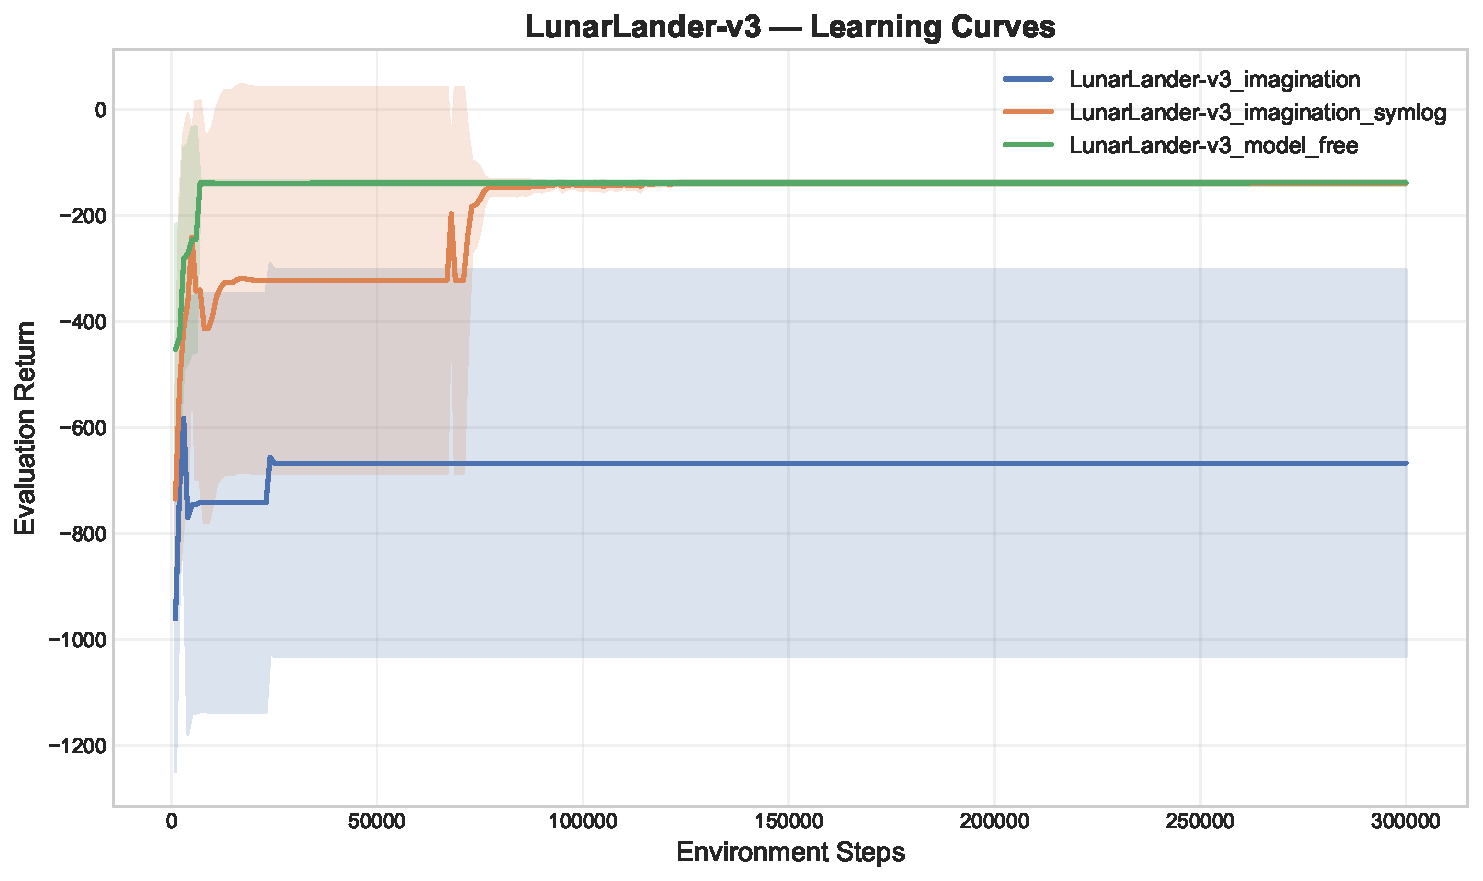
\includegraphics[width=0.85\textwidth]{figures/LunarLander-v3_learning_curves.pdf}
    \caption{LunarLander-v3 learning curves: mean episodic return ($\pm 1$
             standard deviation) over 300\,000 environment steps for each
             agent condition.}
    \label{fig:lunar-learning}
\end{figure}

% ---------------------------------------------------------------
\subsection{Critic Loss Stability}
\label{subsec:lunar-critic}
% ---------------------------------------------------------------

Figure~\ref{fig:lunar-loss} compares the critic loss for the two
imagination-augmented conditions in LunarLander-v3.
Condition~B (standard MSE) undergoes a critic
loss explosion at approximately 100\,000 steps, with the critic loss
reaching the order of $10^{15}$. Condition~C (Symlog MSE) maintains a
stable critic loss throughout the full 300\,000 steps,
with no runaway gradient dynamics.

\begin{figure}[H]
    \centering
    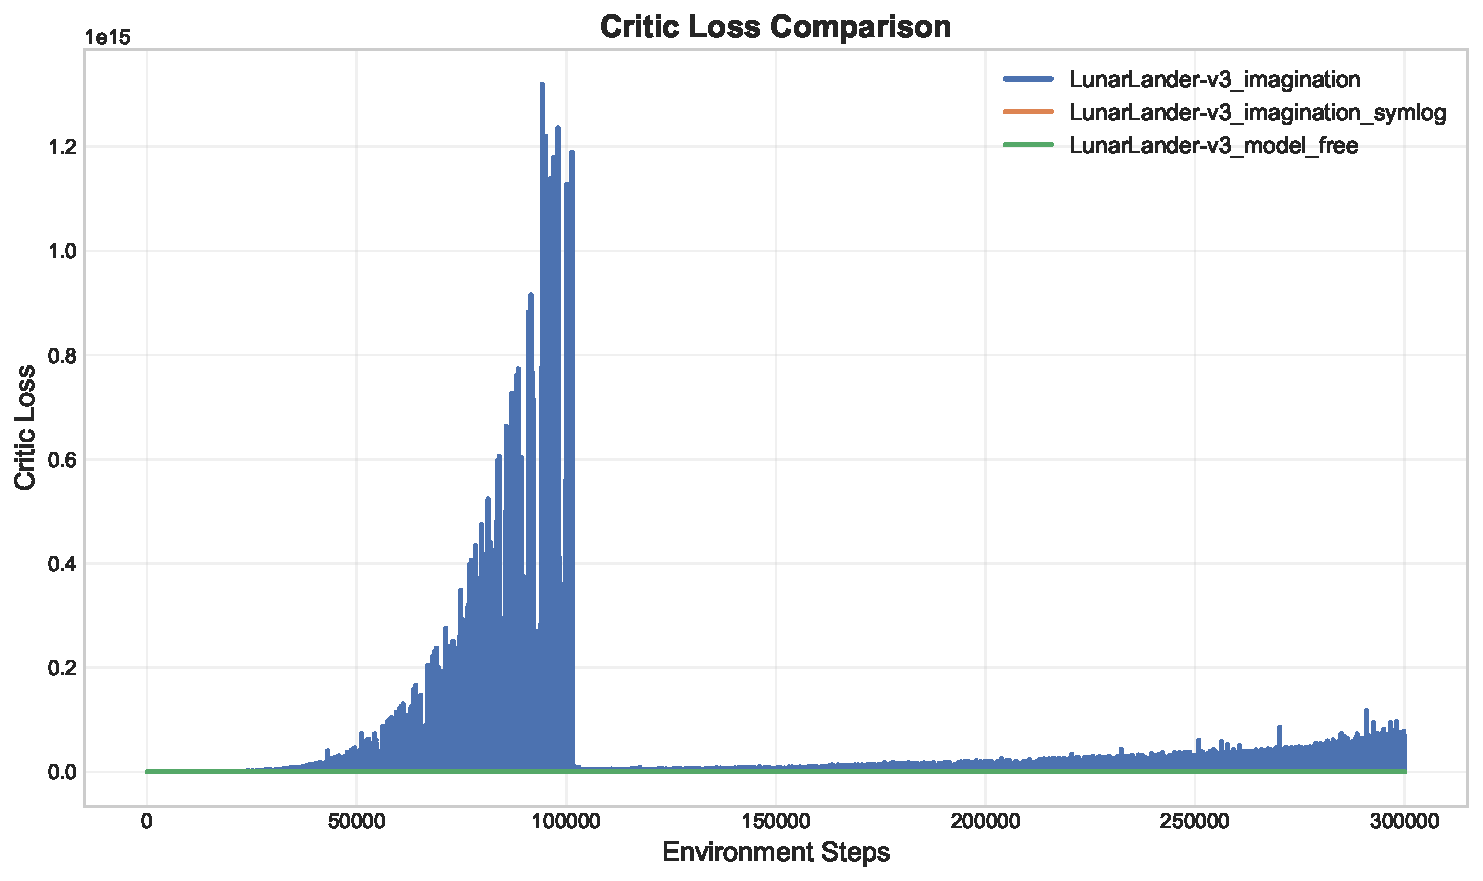
\includegraphics[width=0.85\textwidth]{figures/LunarLander-v3_loss_comparison.pdf}
    \caption{LunarLander-v3 critic loss comparison between the two
             imagination-augmented conditions over 300\,000 environment
             steps. Condition~B explodes to $\sim\!10^{15}$; Condition~C
             remains stable near zero.}
    \label{fig:lunar-loss}
\end{figure}

% ---------------------------------------------------------------
\subsection{World Model Accuracy}
\label{subsec:lunar-wm}
% ---------------------------------------------------------------

Figure~\ref{fig:lunar-wm} presents the world model prediction errors for
LunarLander-v3. The dynamics prediction error is similar for both
imagination-augmented conditions, indicating that both world models acquire
a comparable representation of the environment's transition function.
However, the reward prediction error differs: Condition~B (standard
MSE) exhibits large, fluctuating reward MSE, varying between
0 and approximately 450 MSE throughout training. Condition~C (Symlog MSE)
maintains a near-zero reward prediction error.

\begin{figure}[H]
    \centering
    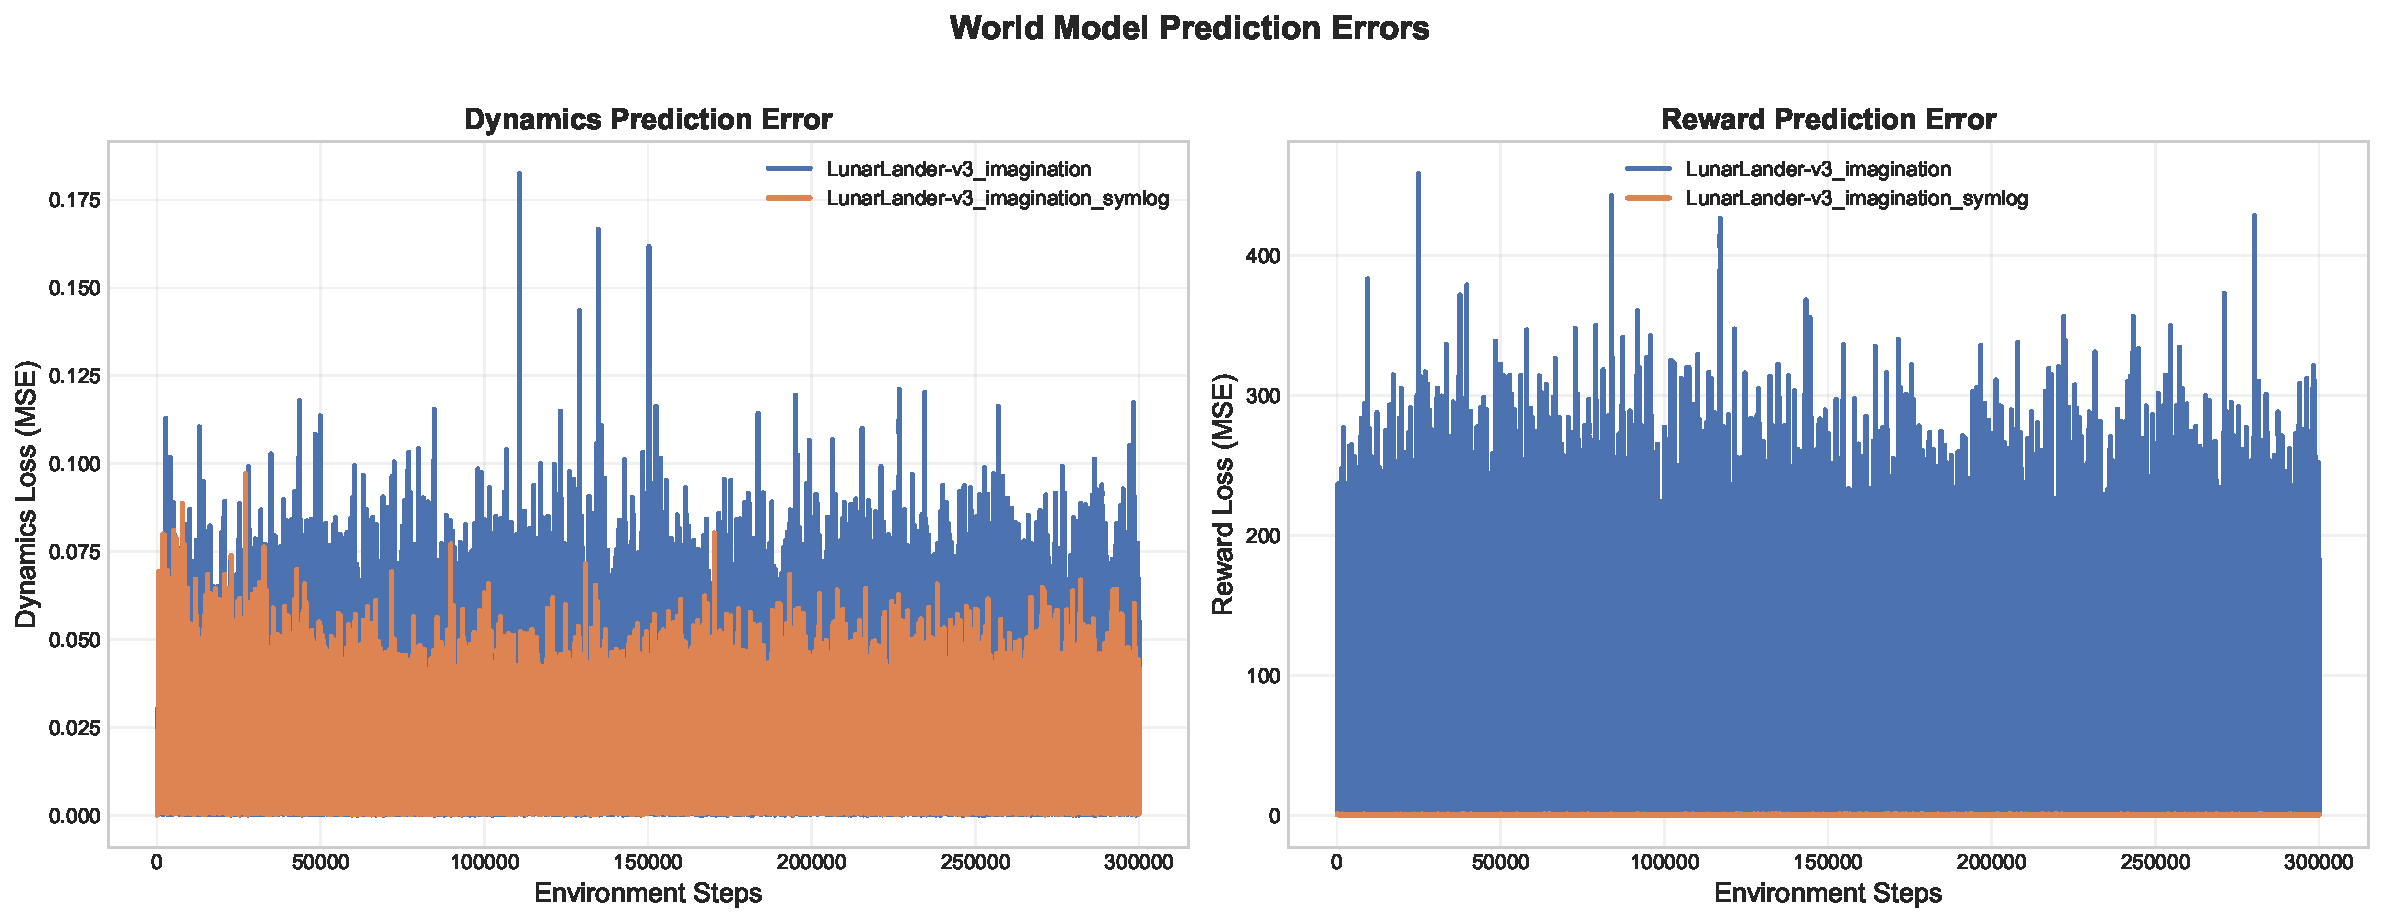
\includegraphics[width=0.85\textwidth]{figures/LunarLander-v3_world_model_error.pdf}
    \caption{LunarLander-v3 world model prediction error: dynamics MSE and
             reward MSE for Conditions~B and~C over 300\,000 environment
             steps.}
    \label{fig:lunar-wm}
\end{figure}


% ================================================================
\section{Comparative Summary}
\label{sec:comparative-summary}
% ================================================================

Table~\ref{tab:results-summary} summarizes the quantitative and qualitative outcomes across the configurations and environments. For each pair, the table reports the approximate final mean episodic return, critic loss stability, and world model reward prediction error stability. The imagination-augmented agent benefits from symlog-transformed losses in both environments, particularly in LunarLander-v3 where the configuration without symlog collapses.

\begin{table}[ht]
    \centering
    \caption{Comparative summary of experimental results across conditions
             and environments.}
    \label{tab:results-summary}
    \begin{tabular}{llccc}
        \toprule
        \textbf{Environment} & \textbf{Condition} &
        \textbf{Final Return} & \textbf{Critic Loss} &
        \textbf{WM Reward Error} \\
        \midrule
        \multirow{3}{*}{CartPole-v1}
            & A: Model-Free       & ${\sim}\,350$ & N/A     & N/A     \\
            & B: Imagination (MSE) & ${\sim}\,400$ & Exploded (${\sim}\!5\!\times\!10^{11}$)
                                                              & Near zero \\
            & C: Imagination (Symlog) & ${\sim}\,430$ & Stable & Near zero \\
        \midrule
        \multirow{3}{*}{LunarLander-v3}
            & A: Model-Free       & ${\sim}\!-140$ & N/A    & N/A     \\
            & B: Imagination (MSE) & ${\sim}\!-1000$ & Exploded (${\sim}\!10^{15}$)
                                                               & Unstable (0 to 450) \\
            & C: Imagination (Symlog) & ${\sim}\!-140$ & Stable & Near zero \\
        \bottomrule
    \end{tabular}
\end{table}


% ================================================================
\section{Summary}
\label{sec:results-summary}
% ================================================================

This chapter presented the experimental results. In CartPole-v1, the imagination-augmented agent with symlog (Condition C) achieved the highest return and maintained stable critic losses, while the standard MSE variant (Condition B) showed late-stage critic loss divergence. In LunarLander-v3, Condition B suffered critic loss divergence and policy collapse, whereas Condition C remained stable. Across both environments, dynamics prediction errors were similar, but reward prediction stability was higher in the symlog configuration. These results are discussed in Chapter~\ref{ch:evaluation}.